A figura \ref{fig:D1_7} representa em diagrama de blocos o modelo de segunda ordem do motor de corrente contínua.

\begin{figure}[ht!]
\center
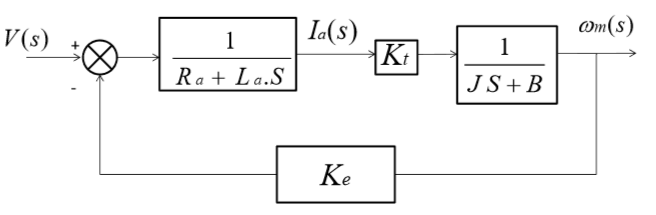
\includegraphics[scale= 0.55]{imagens/diagrama1_7.png}
\caption{\label{fig:D1_7} Modelo de segunda ordem do motor de corrente contínua.}
\caption*{Fonte: MARTINS, cap. 4, eslaide 2.}
\end{figure}


\subsubsection{Resposta da velocidade}

Considerando o diagrama de blocos da figura \ref{fig:D1_7} e  que:

$t \rightarrow \infty$;

$\omega_{m}(\infty) = \omega_{o}K$;

$\omega_{o} = \frac{V}{K_{e}}$;

$k = \frac{\tau_{b}}{\tau_{m}}$.

E os seguintes parâmetros:

$\tau_{b} = \frac{J}{B}$;

$\tau_{m} = \frac{R_{a}J}{K_{e}K_{t}}$;

$\tau_{a} = \frac{L_{a}}{R_{a}}$;

$\gamma_{3} = -\frac{C_{1}}{2} + \sqrt{\frac{C_{1}^{2}}{4} - C_{2}} $;

$\gamma_{4} = -\frac{C_{1}}{2} - \sqrt{\frac{C_{1}^{2}}{4} - C_{2}} $;

$C_{1} = \frac{1}{\tau_{a}} + \frac{1}{\tau_{b}}$

$C_{2} = \frac{1}{\tau_{a}\tau_{b}} + \frac{1}{\tau_{a}\tau_{m}}$;

A equação que modela a resposta da velocidade pode ser representada pela expressão a seguir:
\[\omega_{m}(t) = \omega_{o}K\left[1 + \frac{\gamma_{4}}{\gamma_{3} - \gamma_{4}}e^{\gamma_{3}t} - \frac{\gamma_{3}}{\gamma_{3} - \gamma_{4}}e^{\gamma_{4}t}\right]\]

\subsubsection{Resposta da corrente}

Ainda de acordo com o diagrama de blocos da figura \ref{fig:D1_7}, as considerações do item 2.6.1 e que:

$I_{SC} = \frac{V}{R_{a}}$

Para $t \rightarrow \infty \Rightarrow i_{a}(t) \rightarrow I_{SC}(1 - K)$

A função que expressa a resposta da corrente pode ser dada por:

\[i_{a}(t) = I_{SC}\left[1 - K + \frac{\frac{1}{\tau_{a}} + \gamma_{4} - \gamma_{4}K}{\gamma_{3} - \gamma_{4}}e^{\gamma_{3}t} - \frac{\frac{1}{\tau_{a}} + \gamma_{3} - \gamma_{3}K}{\gamma_{3} - \gamma_{4}}e^{\gamma_{4}t}\right]\]

Finalmente, as formas de onda da corrente e da velocidade para o modelo em questão são ilustradas na figura \ref{fig:G1_72}.

\begin{figure}[ht!]
\center
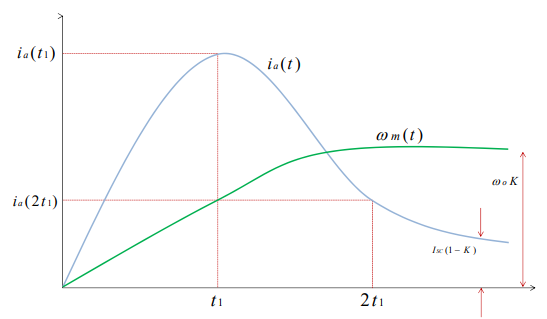
\includegraphics[scale= 0.55]{imagens/grafico1_72.png}
\caption{\label{fig:G1_72} Formas de onda da corrente e da velocidade no motor CC (Regime transitório e permanente) .}
\caption*{Fonte: MARTINS, cap. 4, eslaide 5.}
\end{figure}

Fazendo $\frac{\delta{i_{a}(t_{1}}}{\delta{t}} = 0$, obtém-se o ponto onde a corresnte é máxima.

Dessa forma:
\[ e^{\frac{t_{1}}{\tau_{a}}\left(\tau_{a}\gamma_{3} - \tau_{a}\gamma_{4}\right)} = \frac{\tau_{a}\gamma_{4}\left(1 + \tau_{a}\gamma_{3} - \tau_{a}\gamma_{3}K\right)}{\tau_{a}\gamma_{3}\left(1 + \tau_{a}\gamma_{4} - \tau_{a}\gamma_{4}K\right)}\]

\subsubsection{Procedimento para a medição dos parâmetros do motor de corrente contínua}

Para medir os parâmetros do motor de corrente contínua são empregados os seguintes métodos:

\begin{enumerate}
   \item Levantar as curvas $\omega_{m}(t)$ e i(t) experimentalmente. E a patir delas estabelecer as grandezas.
   
   $t_{1}, i_{t_{1}}, i_{2t_{1}}, I_{SC}(1-K), \omega_{o}K $
   
   \item Seja a relação de Pasek:
   
   \[\frac{i_{2t_{1}}}{i_{t_{1}}} = \frac{i_{t_{1}}}{I_{SC}}\]
   
   Desta forma pode-se determinar $I_{SC}$.
   
   \item Com a relação de $I_{SC}(1-K)$ determina-se o valor de K.
   
   \item Com a relação $I_{SC} = \frac{V}{R_{a}}$ determina-se o valor de $R_{a}$ visto que V é uma variável conhecida a partir dos ensaios.
   
   \item Com a relação $\frac{i_{2t_{1}}}{i_{t_{1}}}$ e com K, encontra-se no ábaco da figura \ref{fig:G1_73} e determina-se o valor de $\frac{\tau_{a}}{\tau_{m}}$.
   
   \item Com $\frac{\tau_{a}}{\tau_{m}}$ e K entra-se no ábaco da figura \ref{fig:G2_73} e determina-se $\frac{t_{1}}{\tau_{a}}$. Como $t_{1}$ é conhecido pode-se encontrar  $\tau_{a}$.
   
   \item Com a relação $\tau_{a} = \frac{L_{a}}{R_{a}}$ determina-se o valor de $L_{a}$.
   
   \item Com o valor de $\omega_{o}K$ e K, $\omega_{o}$ fica determinado.
   
   \item Com a relação de $\omega_{o} = V/K_{e}$, $k_{e}$ e $k_{t}$ ficam determinados.
   
   \item Com a relação $\tau_{a}/\tau_{m}$, $\tau_{m}$ pode ser determinado.
   
   \item Com a relação $\tau_{m} = \frac{R_{a}J}{K_{e}K_{t}}$, o valor de J fica determinado.
   
   \item Com a relação $K = \frac{\tau_{b}}{\tau_{b} + \tau_{m}}$, o valor de $\tau_{b}$ pode ser determinado.
   
   \item Com a relação $\tau_{b} = \frac{J}{B}$, o valor da constante de atrito B é determinado.
   

\end{enumerate}

\begin{figure}[ht!]
\center
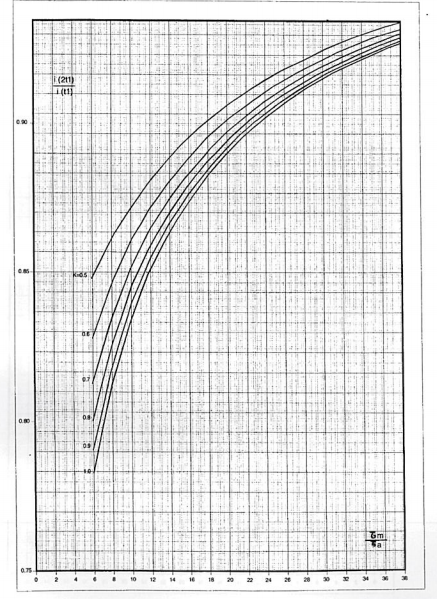
\includegraphics[scale= 0.55]{imagens/grafico1_73.png}
\caption{\label{fig:G1_73} Gráfico relacionando $i(2t_{1})/i(t_{1})$ em função de $\tau_{m}/\tau_{a}$ tendo K como parâmetro.}
\caption*{Fonte: Princípios de acionamento elétrico em corrente contínua (2006).}
\end{figure}

\begin{figure}[ht!]
\center
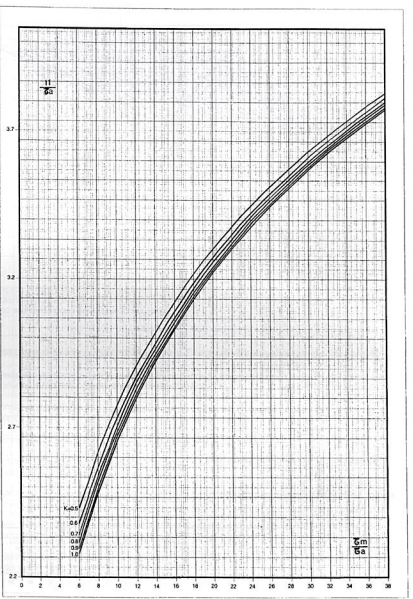
\includegraphics[scale= 0.55]{imagens/grafico2_73.png}
\caption{\label{fig:G2_73} Gráfico relacionando $t_{1}/\tau_{a}$ em função de $\tau_{m}/\tau_{a}$ tendo K como parâmetro.}
\caption*{Fonte: Princípios de acionamento elétrico em corrente contínua (2006) .}
\end{figure}

Os tópicos a seguir referem-se ao estudo da associação dos motores de corrente contínua aos conversores estáticos.

